% Chapter ea: the note of October 20, 2026, assembled for the compendium -- do not edit by hand
\chapter{Detailed derivation of free--free absorption by electron--atom collisions at terahertz frequencies}\label{ea:chapter}
\notedate{October 20, 2026}
\begingroup
\noindent\emph{These notes derive, with every intermediate result written
out, the rate at which an electromagnetic wave of terahertz frequency is
absorbed by free electrons that collide with neutral atoms. They ask whether
the classical absorption kernel, the Lorentz-gas conductivity built on the
momentum-transfer cross section, is accurate at the terahertz frequencies
proposed for reheating the electrons of an electron-beam-pumped KrF laser
gas. The electron is described by exact scattering states of a local
potential that represents the atom, the field is treated to first order, and
the rate follows from the golden rule. Every boxed result is checked
numerically, as Appendix~\ref{ea:app:checks} describes.}

\medskip
\noindent For notation, Gaussian units are used. The
electron has charge $-e$ and mass $m$, and the atom is infinitely heavy and
sits at the origin. A state of momentum $\hbar\kv$ has energy
$E=\hbar^2k^2/2m$ and speed $v=\hbar k/m$. The wave is uniform and linearly
polarized along the unit vector $\ehat$, with amplitude $E_0$ and angular
frequency $\omega$, and $f=\omega/2\pi$ is its frequency. The absorption of one
photon takes the electron from $\hbar\kv$ to $\hbar\kv'$ with
$k'^2=k^2+2m\omega/\hbar$. The temperature of a Maxwell distribution is $T$ and
$u=\hbar\omega/\kB T$. The momentum-transfer cross section is $\sm(E)$, and a
cross section with a subscript $+$ or $-$ is the free--free cross section for
absorption or stimulated emission per unit photon flux, defined in
Sec.~\ref{ea:sec:cross}. The numbers are computed in atomic units, $\hbar=m=e=1$,
with the bohr $a_0$ and the hartree $E_h=27.211$~eV. A boxed equation is a
result that is checked.


\section{Why the atoms matter}
\label{ea:sec:why}

{\noindent}(1) Inverse bremsstrahlung, the absorption of a wave by electrons
that scatter on ions, heats laser plasmas \cite{ea:Atzeni2004}. In the gas of an electron-beam-pumped
KrF laser the electron density is $10^{19}$ to $2.7\times10^{21}$~m$^{-3}$
against an atom density of $2.4\times10^{25}$ to $4.9\times10^{25}$~m$^{-3}$,
so that there are $9\times10^3$ to $5\times10^6$ atoms for every ion. The
Coulomb cross section is larger by orders of magnitude, however, and
Sec.~\ref{ea:sec:ei} finds the regime in which each kind of collision dominates
the absorption. Away from the coldest and densest afterglow the atoms win.

{\noindent}(2) Free--free absorption on neutral atoms has been computed from
phase shifts for the negative hydrogen ion \cite{ea:OhmuraOhmura1960} and for
other atoms \cite{ea:Geltman1973}, and with the multichannel R-matrix method for
argon \cite{ea:BellBerrington1987}. Its inverse, the neutral bremsstrahlung, has
been measured \cite{ea:TaylorCaledonia1969,ea:Ranson1977} and explains part of the
electroluminescence of two-phase argon detectors \cite{ea:Buzulutskov2018}.

{\noindent}(3) Proposals to reheat the electrons of the laser gas with a
terahertz wave compute its absorption length with the classical kernel of the
Lorentz gas. That kernel is the
conductivity of electrons that scatter off heavy atoms with the energy
dependent collision frequency $\nu(v)=N\sm(v)v$, derived in
Sec.~\ref{ea:sec:classical}. It treats the electron as a classical particle that
absorbs energy continuously. Two quantum effects are missing from it. The
first is the ratio $u=\hbar\omega/\kB T$, which is $0.16$ at 1~THz and $4.5$
at the 28.3~THz of a CO$_2$ laser for electrons at the gas temperature of
300~K. The second is the structure of $\sm(E)$. Argon and krypton have a
Ramsauer--Townsend window in which $\sm$ falls from its value at 1~meV by a
factor of 82 in argon and 330 in krypton, to minima at 0.25 and 0.51~eV in the
LXCat sets, and a photon of 28.3~THz carries 0.117~eV. Table~\ref{ea:tab:scales}
lists the photon energy and $u$ at the frequencies used below.

\begin{table}[ht]
\caption{Photon energy $\hbar\omega$, the ratio $u=\hbar\omega/\kB T$ and the
stimulated-emission factor $(1-e^{-u})/u$ at 300~K, and $u$ for electrons at
0.63~eV.}
\label{ea:tab:scales}
\begin{center}
\begin{tabular}{lcccc}
\toprule
$f$ (THz) & $\hbar\omega$ (meV) & $u$, 300~K & $(1-e^{-u})/u$, 300~K & $u$, 0.63~eV\\
\midrule
\tabinput{chapters/ea/tab_scales.tex}
\bottomrule
\end{tabular}
\end{center}
\end{table}

{\noindent}(4) The question is the error of the classical kernel at 3 to
28~THz in two fills of the laser gas, Ne/Kr/F$_2$ = 0.948/0.05/0.002 at
2~atm and Ar/Kr/F$_2$ = 0.597/0.40/0.003 at 1~atm. The kernel is good enough
if the error is below 5\,\% in the band of 0.3 to 4~THz proposed for reheating.
Sections~\ref{ea:sec:ham} to~\ref{ea:sec:detailed} derive the quantum free--free
cross section of one electron and one atom exactly within a one-body model.
Section~\ref{ea:sec:soft} finds its soft-photon and classical limits, and
Sec.~\ref{ea:sec:exact} two limits in which it is known in closed form at any
photon energy. Sections~\ref{ea:sec:models} and~\ref{ea:sec:thermal} evaluate it for
model potentials fitted to the measured cross sections of neon, argon and
krypton. The answer is in Sec.~\ref{ea:sec:thermal} and in the Summary.

\section{The Hamiltonian}
\label{ea:sec:ham}

\subsection{One electron and one atom}
{\noindent}(1) The atom is represented by a local central potential $V(r)$
that acts on the scattering electron,
\begin{equation}
H_0=\frac{p^2}{2m}+V(r),\qquad
V(r)\to-\frac{\alpha_de^2}{2r^4}\quad(r\to\infty),
\label{ea:eq:H0}
\end{equation}
where $\alpha_d$ is the static dipole polarizability of the atom. At short
range $V$ contains the screened attraction of the nucleus and the repulsion
that the Pauli principle produces. In the one-body model the latter appears
because the occupied orbitals of the atom are bound states of the same
potential, so that the scattering states are orthogonal to them. The models
of Sec.~\ref{ea:sec:models} are of this kind.

{\noindent}(2) The atom is infinitely heavy. Its recoil changes the electron
energy by a fraction of order $m/M$, which is $1.4\times10^{-5}$ for argon,
and is neglected. Exchange between the scattering electron and the atomic
electrons, and the excitation of the atom, are outside the model. The second
needs at least 11.5~eV in argon and 9.9~eV in krypton and is closed for the
electrons that absorb terahertz photons.

\subsection{The wave}
{\noindent}(1) The wave has the field $\Ev(t)=E_0\ehat\cos\omega t$. At 1~THz
its wavelength is 0.3~mm and at 28.3~THz it is 10.6~$\mu$m. A collision takes
place within a few hundred $a_0$ of the atom, so the field is uniform over it
and the dipole approximation holds. In the length gauge the potential energy of
the charge $-e$ in the field is $e\Ev(t)\cdot\rv$, and
\begin{equation}
H(t)=H_0+eE_0\cos(\omega t)\,\ehat\cdot\rv
=H_0+\frac{eE_0}{2}\,\ehat\cdot\rv\,\big(e^{-i\omega t}+e^{i\omega t}\big).
\label{ea:eq:H}
\end{equation}
The term with $e^{-i\omega t}$ absorbs a photon and the term with
$e^{i\omega t}$ emits one.

{\noindent}(2) The field is weak when the quiver amplitude
$a=eE_0/m\omega^2$ is small against the wavelength of the electron. The
criterion and its numbers are in Sec.~\ref{ea:sec:strong}. In the weak field the
golden rule to first order in $E_0$ describes the absorption of one photon.

\subsection{The response of the atom to the wave}
\label{ea:sec:pb}
{\noindent}(1) The wave also polarizes the atom. Its induced dipole is
$\alpha_d\Ev(t)$, since $\hbar\omega$ is far below the excitation energies of
the atom. The electrostatic potential of a dipole $\mathbf d$ at the origin is
$\mathbf d\cdot\rv/r^3$, so the electron acquires the potential energy
$-e\alpha_d\Ev(t)\cdot\rv/r^3$. Together with Eq.~\eqref{ea:eq:H} the
interaction with the wave becomes
\begin{equation}
e\Ev(t)\cdot\rv\Big(1-\frac{\alpha_d}{r^3}\Big).
\label{ea:eq:pb-op}
\end{equation}
The second term is the polarization bremsstrahlung of the atom, the photon
absorbed through the dipole of the atom rather than through the electron.
Inside the atom the field of the dipole is screened, so the term is cut off
there. Section~\ref{ea:sec:pbnum} computes its effect with the same cut-off as the
polarization potential, and finds it below 0.7\,\% up to 3~THz. Until then it
is left out.

\section{The golden-rule cross section between exact scattering states}
\label{ea:sec:cross}

\subsection{The scattering states}
{\noindent}(1) The scattering states of $H_0$ with energy $E=\hbar^2k^2/2m$
are normalized to $\langle\psi_{\kv}|\psi_{\kv'}\rangle=\delta^3(\kv-\kv')$.
In partial waves,
\begin{equation}
\psi^{(\pm)}_{\kv}(\rv)=(2\pi)^{-3/2}\sum_{l=0}^\infty(2l+1)\,i^l
e^{\pm i\delta_l}\,\frac{u_{kl}(r)}{kr}\,P_l(\hat\kv\cdot\hat\rv),
\label{ea:eq:pw}
\end{equation}
where $u_{kl}$ is the real regular solution of the radial equation
\begin{equation}
u_{kl}''+\Big[k^2-U(r)-\frac{l(l+1)}{r^2}\Big]u_{kl}=0,\qquad
U(r)=\frac{2mV(r)}{\hbar^2},
\label{ea:eq:radial}
\end{equation}
normalized to unit amplitude,
$u_{kl}\to\sin(kr-l\pi/2+\delta_l)$ as $r\to\infty$, and $\delta_l(k)$ is
the phase shift. For $V=0$ the radial function is the Riccati--Bessel
function $\hat\jmath_l(kr)=kr\,j_l(kr)$, and Eq.~\eqref{ea:eq:pw} is the
expansion of the plane wave $(2\pi)^{-3/2}e^{i\kv\cdot\rv}$. The state
$\psi^{(+)}$ has an outgoing scattered wave and is the initial state. The
state $\psi^{(-)}$, with an incoming scattered wave, is the final state of an
electron detected in the direction $\hat\kv'$.

{\noindent}(2) With $P_l(\hat\kv\cdot\hat\rv)=\frac{4\pi}{2l+1}\sum_m
Y^*_{lm}(\hat\kv)Y_{lm}(\hat\rv)$,
\begin{equation}
\psi^{(\pm)}_{\kv}(\rv)=(2\pi)^{-3/2}\,\frac{4\pi}{kr}\sum_{lm}i^le^{\pm i\delta_l}
u_{kl}(r)\,Y^*_{lm}(\hat\kv)\,Y_{lm}(\hat\rv).
\label{ea:eq:pw-ylm}
\end{equation}

\subsection{The matrix element}
{\noindent}(1) The absorption term of Eq.~\eqref{ea:eq:H} has the matrix element
$(eE_0/2)M$ with $M=\langle\psi^{(-)}_{\kv'}|\ehat\cdot\rv|\psi^{(+)}_{\kv}\rangle$.
The complex conjugate of Eq.~\eqref{ea:eq:pw-ylm} for the final state has the
factors $(-i)^{l'}e^{+i\delta'_{l'}}Y_{l'm'}(\hat\kv')Y^*_{l'm'}(\hat\rv)$,
with $\delta'_{l'}=\delta_{l'}(k')$. The factor $r^2$ of $\dd^3r$ cancels the
two factors $1/r$, and
\begin{equation}
M=\frac{(4\pi)^2}{(2\pi)^3kk'}\sum_{lm,l'm'}(-i)^{l'}i^l
e^{i(\delta_l+\delta'_{l'})}\,Y_{l'm'}(\hat\kv')Y^*_{lm}(\hat\kv)\,
\langle l'm'|\ehat\cdot\hat\rv|lm\rangle\,R_{l\to l'},
\label{ea:eq:M}
\end{equation}
with the angular matrix element
$\langle l'm'|\ehat\cdot\hat\rv|lm\rangle=\int Y^*_{l'm'}\,\ehat\cdot\hat\rv\,
Y_{lm}\,\dd\Omega$ and the radial integral
\begin{equation}
R_{l\to l'}=\int_0^\infty u_{k'l'}(r)\,r\,u_{kl}(r)\,\dd r .
\label{ea:eq:Rlen}
\end{equation}
The integrand grows like $r$ at large $r$, and $R_{l\to l'}$ is defined with
the convergence factor $e^{-\eta r}$ and $\eta\to0^+$. Section~\ref{ea:sec:forms}
replaces it by an absolutely convergent integral.

{\noindent}(2) The angular matrix element vanishes unless $l'=l\pm1$, the
dipole selection rule. Appendix~\ref{ea:app:angular} sums its square over $m$
and $m'$,
\begin{equation}
\sum_{mm'}|\langle l+1,m'|\ehat\cdot\hat\rv|lm\rangle|^2=\frac{l+1}{3},\qquad
\sum_{mm'}|\langle l-1,m'|\ehat\cdot\hat\rv|lm\rangle|^2=\frac l3 .
\label{ea:eq:angsum}
\end{equation}

\subsection{The rate and its average over directions}
{\noindent}(1) The golden rule gives the rate of absorption from the state
$\psi^{(+)}_{\kv}$ into all final directions,
\begin{equation}
W_+=\frac{2\pi}{\hbar}\Big(\frac{eE_0}{2}\Big)^2\int\dd^3k'\,|M|^2\,
\delta\Big(\frac{\hbar^2k'^2}{2m}-\frac{\hbar^2k^2}{2m}-\hbar\omega\Big).
\end{equation}

{\noindent}(2) The electrons of a gas move in all directions, so $W_+$ is
averaged over $\hat\kv$. The integral over $\hat\kv'$ and the average over
$\hat\kv$ use the orthonormality of the $Y_{lm}$,
$\int Y_{l'm'}(\hat\kv')Y^*_{l''m''}(\hat\kv')\dd\Omega'=\delta_{l'l''}\delta_{m'm''}$
and $\frac1{4\pi}\int Y^*_{lm}(\hat\kv)Y_{\tilde l\tilde m}(\hat\kv)\dd\Omega
=\delta_{l\tilde l}\delta_{m\tilde m}/4\pi$. The cross terms between different
pairs $(l,l')$ vanish, the phases drop out, and with Eq.~\eqref{ea:eq:angsum}
\begin{equation}
\frac1{4\pi}\int\dd\Omega\int\dd\Omega'\,|M|^2
=\frac{(4\pi)^4}{(2\pi)^6k^2k'^2}\,\frac1{4\pi}\,\frac{S}{3}
=\frac{S}{3\pi^3k^2k'^2},
\label{ea:eq:Mavg}
\end{equation}
\begin{equation}
S=\sum_{l=0}^\infty\Big[(l+1)\,R_{l\to l+1}^2+l\,R_{l\to l-1}^2\Big].
\label{ea:eq:S}
\end{equation}

{\noindent}(3) The energy delta function contributes
$\int k'^2\dd k'\,\delta(\hbar^2k'^2/2m-E-\hbar\omega)=mk'/\hbar^2$. The
averaged rate is
\begin{equation}
\langle W_+\rangle=\frac{2\pi}{\hbar}\,\frac{e^2E_0^2}{4}\,\frac{mk'}{\hbar^2}\,
\frac{S}{3\pi^3k^2k'^2}=\frac{e^2E_0^2\,m\,S}{6\pi^2\hbar^3k^2k'} .
\end{equation}

\subsection{The cross section per photon flux}
{\noindent}(1) The state $\psi^{(+)}_{\kv}$ carries the incident flux
$(2\pi)^{-3}\hbar k/m$ of electrons, and the wave carries the flux
$\Phi=I/\hbar\omega$ of photons with $I=cE_0^2/8\pi$. The free--free cross
section for absorption is the rate divided by both fluxes,
$\sigma_+=\langle W_+\rangle/[(2\pi)^{-3}(\hbar k/m)\Phi]$. With
$(2\pi)^3\cdot8\pi/6\pi^2=32\pi^2/3$,
\begin{equation}
\boxed{\;\sigma_+(k\to k')=\frac{32\pi^2}{3}\,\frac{e^2m^2\omega}{\hbar^3c}\,
\frac{S}{k^3k'},\qquad \hbar k'=(\hbar^2k^2+2m\hbar\omega)^{1/2}.\;}
\label{ea:eq:sigplus}
\end{equation}
It has the dimension length$^4\times$time. An electron of speed $v$ among $N$
atoms per unit volume, in the photon flux $\Phi$, absorbs at the rate
$N\Phi v\sigma_+$.

{\noindent}(2) In the first Born approximation the radial functions are
$\hat\jmath_l$ and Eq.~\eqref{ea:eq:sigplus} must equal the one-photon limit of
the cross section of Bunkin and Fedorov \cite{ea:BunkinFedorov1966}, with
$J_1^2(x)\simeq x^2/4$, divided by $\Phi$. The check script compares the two
for a Gaussian potential and finds agreement to $10^{-14}$, which tests the
factor $32\pi^2/3$ and the angular sums together.

\subsection{Length, velocity and acceleration forms}
\label{ea:sec:forms}
{\noindent}(1) For eigenstates of $H_0$ the commutators
$[H_0,\rv]=-i\hbar\pv/m$ and $[H_0,\pv]=i\hbar\nabla V$ give
$[H_0,[H_0,\rv]]=(\hbar^2/m)\nabla V$. Between states that differ in energy by
$\hbar\omega$ the double commutator is $(\hbar\omega)^2$ times the matrix
element of $\rv$, so
\begin{equation}
\langle f|\rv|i\rangle=\frac{-i}{m\omega}\langle f|\pv|i\rangle
=\frac{1}{m\omega^2}\langle f|\nabla V|i\rangle .
\label{ea:eq:forms}
\end{equation}
For scattering states the boundary terms at infinity oscillate and vanish with
the convergence factor $e^{-\eta r}$, so the identities hold for the
regularized integrals of Eq.~\eqref{ea:eq:Rlen}.

{\noindent}(2) Since $\nabla V=V'(r)\hat\rv$ has the same angular structure as
$\rv=r\hat\rv$, the identity holds partial wave by partial wave,
\begin{equation}
\boxed{\;R_{l\to l'}=\frac{1}{m\omega^2}\int_0^\infty u_{k'l'}(r)\,V'(r)\,u_{kl}(r)\,\dd r .\;}
\label{ea:eq:Racc}
\end{equation}
The acceleration form converges absolutely when $V'$ falls faster than $1/r$,
as the $r^{-5}$ of the polarization tail does, and the numerics use it. The
form makes plain that the photon is absorbed where the electron is
accelerated, near the atom. The check script verifies Eq.~\eqref{ea:eq:Racc}
against the closed form of the length integral in the zero-range limit of
Sec.~\ref{ea:sec:zerorange}.

\section{Emission, detailed balance and the absorption coefficient}
\label{ea:sec:detailed}

\subsection{Stimulated emission and detailed balance}
{\noindent}(1) The term with $e^{i\omega t}$ in Eq.~\eqref{ea:eq:H} takes an
electron from $\hbar\kv'$ to $\hbar\kv$ and adds a photon to the wave. The
same steps give its cross section per photon flux, with $k$ and $k'$
exchanged in the prefactor,
$\sigma_-(k'\to k)=(32\pi^2e^2m^2\omega/3\hbar^3c)\,S'/(k'^3k)$. Here $S'$ has
the radial integrals $R'_{l\to l'}=\int u_{kl'}\,r\,u_{k'l}\,\dd r=R_{l'\to l}$.
Shifting the summation index in each of the two sums of Eq.~\eqref{ea:eq:S}
shows $S'=S$. Hence
\begin{equation}
\boxed{\;k^2\,\sigma_+(k\to k')=k'^2\,\sigma_-(k'\to k).\;}
\label{ea:eq:db}
\end{equation}
This is the principle of detailed balance for free--free transitions.

\subsection{The absorption coefficient}
{\noindent}(1) Let $g(E)\dd E$ be the fraction of electrons with energy in
$\dd E$, for an isotropic distribution normalized to $\int g\,\dd E=1$, and
let $\sigma_-(E)$ denote the emission cross section from $E$ to $E-\hbar\omega$,
zero for $E<\hbar\omega$. The wave loses photons at the rate
$n_eN\Phi\int g\,v(\sigma_+-\sigma_-)\dd E$ per unit volume, so its intensity
decays with the coefficient
\begin{equation}
\boxed{\;\kappa=n_eN\int_0^\infty g(E)\,v(E)\big[\sigma_+(E)-\sigma_-(E)\big]\dd E .\;}
\label{ea:eq:kappa-gen}
\end{equation}

{\noindent}(2) Shift the emission integral to $E=E''+\hbar\omega$ and use
Eq.~\eqref{ea:eq:db}, $\sigma_-(E''+\hbar\omega)=[E''/(E''+\hbar\omega)]\,\sigma_+(E'')$.
For the Maxwell distribution
$g(E)=2\pi^{-1/2}(\kB T)^{-3/2}E^{1/2}e^{-E/\kB T}$,
\begin{equation}
g(E''+\hbar\omega)\,v(E''+\hbar\omega)\,\frac{E''}{E''+\hbar\omega}
=e^{-u}\,g(E'')\,v(E''),
\end{equation}
since $g\,v$ is proportional to $E\,e^{-E/\kB T}$. Therefore
\begin{equation}
\boxed{\;\kappa=n_eN\,(1-e^{-u})\int_0^\infty g(E)\,v(E)\,\sigma_+(E)\,\dd E
\qquad\text{(Maxwell electrons)}.\;}
\label{ea:eq:kappa-mb}
\end{equation}
Stimulated emission reduces the absorption by the factor $1-e^{-u}$, as it
does for ions \cite{ea:KarzasLatter1961}.

\subsection{The kinetic equation and its Fokker--Planck limit}
\label{ea:sec:kinetic}
{\noindent}(1) Let $n(E)\dd E$ be the number of electrons per unit volume in
$\dd E$, and write $n=n_eE^{1/2}F(E)$ with $\int E^{1/2}F\,\dd E=1$, the
normalization of the two-term Boltzmann codes \cite{ea:HagelaarPitchford2005}.
An electron at $E$ climbs to $E+\hbar\omega$ at the rate
$W_+(E)=N\Phi v\sigma_+(E)$ and falls to $E-\hbar\omega$ at the rate
$W_-(E)=N\Phi v\sigma_-(E)$. The master equation for the distribution is
\begin{equation}
\frac{\partial n(E)}{\partial t}=W_+(E-\hbar\omega)n(E-\hbar\omega)
+W_-(E+\hbar\omega)n(E+\hbar\omega)-\big[W_+(E)+W_-(E)\big]n(E).
\label{ea:eq:master}
\end{equation}

{\noindent}(2) Detailed balance, Eq.~\eqref{ea:eq:db}, makes the two rates that
connect $E$ and $E+\hbar\omega$ equal after weighting with $E^{1/2}$,
\begin{equation}
W_+(E)\,E^{1/2}=W_-(E+\hbar\omega)\,(E+\hbar\omega)^{1/2}
=N\Phi\Big(\frac2m\Big)^{1/2}E\,\sigma_+(E)\equiv\mathcal Q\Big(E+\frac{\hbar\omega}2\Big).
\end{equation}
Dividing Eq.~\eqref{ea:eq:master} by $n_e$ gives the jump operator in
conservation form,
\begin{equation}
\boxed{\;\frac{\partial(E^{1/2}F)}{\partial t}
=\mathcal Q\Big(E+\frac{\hbar\omega}2\Big)\big[F(E+\hbar\omega)-F(E)\big]
-\mathcal Q\Big(E-\frac{\hbar\omega}2\Big)\big[F(E)-F(E-\hbar\omega)\big].\;}
\label{ea:eq:jump}
\end{equation}
The right side is a difference of two fluxes through the energies
$E\pm\hbar\omega/2$, so the operator conserves the number of electrons.

{\noindent}(3) When $\hbar\omega$ is small against the scale on which $F$ and
$\mathcal Q$ vary, each bracket is $\hbar\omega\,\partial F/\partial E$ at the
midpoint, and the difference of the two fluxes is $\hbar\omega$ times their
derivative,
\begin{equation}
\frac{\partial(E^{1/2}F)}{\partial t}=\frac{\partial}{\partial E}
\Big[\mathcal D(E)\,\frac{\partial F}{\partial E}\Big]+O\big((\hbar\omega)^4\big),
\qquad \mathcal D=(\hbar\omega)^2\mathcal Q(E).
\end{equation}
With the soft-photon cross section of Sec.~\ref{ea:sec:soft},
$\sigma_+=4\pi e^2v^2\sm/3c\hbar\omega^3$, and $\Phi=cE_0^2/8\pi\hbar\omega$,
\begin{equation}
\boxed{\;\mathcal D(E)=\frac{2}{3}\,\frac{e^2E_{\rm rms}^2}{m\omega^2}\,
N\Big(\frac2m\Big)^{1/2}E^2\,\sm(E),\qquad E_{\rm rms}^2=\frac{E_0^2}{2}.\;}
\label{ea:eq:Dfp}
\end{equation}
This is the field term of the two-term Boltzmann equation in a high-frequency
field \cite{ea:HagelaarPitchford2005} in the limit $\omega\gg\nu$. There the field
diffusion is $\propto E_{\rm rms}^2\,\epsilon\,\sigma/[\sigma^2+(\omega/N)^2/\gamma^2\epsilon]$
and tends to $E_{\rm rms}^2\epsilon^2\sigma/\omega^2$, the dependence $E^2\sm$ of
Eq.~\eqref{ea:eq:Dfp}. The check script confirms that both give the same heating
rate. Equation~\eqref{ea:eq:jump} is therefore the form that a two-term code should
use when $\hbar\omega$ is not small against the energies of the electrons.

\section{The soft-photon limit}
\label{ea:sec:soft}

\subsection{The force identity}
\label{ea:sec:force}
{\noindent}(1) As $\omega\to0$ the final state approaches the initial one, and
Eq.~\eqref{ea:eq:Racc} needs the integral of $V'$ between two states of the same
energy and neighbouring $l$. It is fixed by the phase shifts alone. Write
$u_l=u_{kl}$, $u_{l+1}=u_{k,l+1}$ and $A_l=l(l+1)/r^2$, so that
$u_l''=(A_l+U-k^2)u_l$ by Eq.~\eqref{ea:eq:radial}, and define
\begin{equation}
P=u_{l+1}u_l,\qquad h=u_{l+1}'u_l',\qquad g=u_{l+1}'u_l-u_{l+1}u_l' .
\end{equation}

{\noindent}(2) The radial equations give
$h'=(U-k^2)P'+A_{l+1}u_{l+1}u_l'+A_lu_{l+1}'u_l$. With
$(U-k^2)P'=[(U-k^2)P]'-U'P$ this is
\begin{equation}
U'P=\big[(U-k^2)P\big]'-h'+A_{l+1}u_{l+1}u_l'+A_lu_{l+1}'u_l .
\end{equation}

{\noindent}(3) The two centrifugal terms are
$\frac{l+1}{r^2}\big[(l+2)u_{l+1}u_l'+l\,u_{l+1}'u_l\big]
=\frac{l+1}{r^2}\big[(l+1)P'-g\big]$.
The equations for $u_l$ and $u_{l+1}$ also give $g'=(A_{l+1}-A_l)P=2(l+1)P/r^2$.
Hence
\begin{equation}
\frac{(l+1)^2P'}{r^2}=\Big[\frac{(l+1)^2P}{r^2}\Big]'+\frac{2(l+1)^2P}{r^3}
=\Big[\frac{(l+1)^2P}{r^2}\Big]'+\frac{(l+1)g'}{r},
\end{equation}
and $(l+1)g'/r-(l+1)g/r^2=(l+1)(g/r)'$. Every term is a derivative,
\begin{equation}
U'(r)\,u_{l+1}u_l=\frac{\dd}{\dd r}\Big[(U-k^2)P-h+\frac{(l+1)^2P}{r^2}+\frac{(l+1)g}{r}\Big].
\label{ea:eq:totalder}
\end{equation}

{\noindent}(4) At $r=0$ the regular solutions behave as $r^{l+1}$ and $r^{l+2}$,
so $P\sim r^{2l+3}$, $h$, $P/r^2$ and $g/r$ all $\sim r^{2l+1}$, and the
bracket vanishes for a potential less singular than $r^{-3}$. Where $U$ has
fallen off, $u_l=\sin\varphi$ and $u_{l+1}=-\cos(\varphi+\Delta)$ with
$\varphi=kr-l\pi/2+\delta_l$ and $\Delta=\delta_{l+1}-\delta_l$. Then $g\to
k\cos\Delta$ is bounded, the terms with $1/r$ and $1/r^2$ vanish, and
\begin{equation}
-k^2P-h=k^2\big[\sin\varphi\cos(\varphi+\Delta)-\cos\varphi\sin(\varphi+\Delta)\big]
=-k^2\sin\Delta,
\end{equation}
a constant. Integrating Eq.~\eqref{ea:eq:totalder} from 0 to $\infty$ and
returning to $V=\hbar^2U/2m$,
\begin{equation}
\boxed{\;\int_0^\infty u_{k,l+1}\,V'(r)\,u_{kl}\,\dd r=\frac{\hbar^2k^2}{2m}\,
\sin(\delta_l-\delta_{l+1}).\;}
\label{ea:eq:force}
\end{equation}
The check script verifies it for the deep models of argon and krypton of
Sec.~\ref{ea:sec:models} at $ka_0\ge0.05$, to $10^{-4}$ for each $l\le2$ and to
$4\times10^{-6}$ for the sum over $l\le9$ weighted with $l+1$, as the integrals
enter the cross sections below. The higher partial waves at small $k$ carry
integrals of $10^{-7}$ and less, which the integration resolves only to a few
per cent.

\subsection{The soft-photon cross section}
{\noindent}(1) Insert Eq.~\eqref{ea:eq:force} into Eq.~\eqref{ea:eq:Racc} at
$k'=k$. The terms with $l\to l+1$ and $l\to l-1$ of Eq.~\eqref{ea:eq:S} give the
same sum after a shift of the index,
\begin{equation}
S\to\Big(\frac{\hbar^2k^2}{2m^2\omega^2}\Big)^2\,2\sum_l(l+1)\sin^2(\delta_l-\delta_{l+1})
=\frac{\hbar^4k^6}{8\pi m^4\omega^4}\,\sm(E),
\end{equation}
with the momentum-transfer cross section of Appendix~\ref{ea:app:angular},
\begin{equation}
\sm(E)=\int(1-\cos\theta)\frac{\dd\sigma}{\dd\Omega}\dd\Omega
=\frac{4\pi}{k^2}\sum_{l=0}^\infty(l+1)\sin^2(\delta_l-\delta_{l+1}).
\label{ea:eq:sigmam}
\end{equation}

{\noindent}(2) Equation~\eqref{ea:eq:sigplus} becomes
\begin{equation}
\boxed{\;\sigma_+\to\sigma_+^{\rm soft}=\frac{4\pi}{3}\,\frac{e^2v^2}{c\hbar\omega^3}\,\sm(E)
\qquad(\hbar\omega\ll E).\;}
\label{ea:eq:soft}
\end{equation}
This is the content of the low-energy theorem of Low \cite{ea:Low1958} for
potential scattering. Kroll and Watson \cite{ea:KrollWatson1973} wrote it, angle by
angle, as $(k'/k)(\Qv\cdot\avea)^2/4$ times the elastic cross section, where
$\Qv=\kv-\kv'$ and $\avea=eE_0\ehat/m\omega^2$. The average of
$(\Qv\cdot\ehat)^2$ over directions is $Q^2/3$, and $Q^2=2k^2(1-\cos\theta)$
turns the elastic cross section into $\sm$, which is Eq.~\eqref{ea:eq:soft}.

{\noindent}(3) The literature on neutral bremsstrahlung, the emission that
corresponds to this absorption, is divided on this point. Buzulutskov et
al.~\cite{ea:Buzulutskov2018} report two opinions, the integral elastic cross
section, used by Kas'yanov and Starostin \cite{ea:KasyanovStarostin1965} among
others, and the momentum-transfer cross section, used by Dalgarno and Lane
\cite{ea:DalgarnoLane1966} among others, and they adopt the elastic one. The
force identity decides for $\sm$. The two differ where the scattering is
anisotropic, most of all in the Ramsauer windows. At the minimum of the deep
models of Sec.~\ref{ea:sec:models} the elastic cross section is 3.8 times $\sm$
in argon and 6.6 times in krypton.

\subsection{The classical limit is the Lorentz gas}
\label{ea:sec:classical}
{\noindent}(1) The classical kernel is the conductivity of the Lorentz gas. Expand the distribution of velocities as
$f_0(v)+(\vv\cdot\ehat/v)f_1(v,t)$. The force on an electron is $-e\Ev$, and
heavy scatterers relax the anisotropic part at the rate $\nu(v)=N\sm v$. The
Boltzmann equation gives for $f_1=\Real[\hat f_1e^{-i\omega t}]$
\begin{equation}
(\nu-i\omega)\hat f_1=\frac{eE_0}{m}\frac{\partial f_0}{\partial v}.
\end{equation}

{\noindent}(2) The current along $\ehat$ is $-e\int v\cos^2\theta\,f_1\,\dd^3v
=-(4\pi e/3)\int v^3f_1\,\dd v$, and with $\int4\pi v^2f_0\,\dd v=n_e$ the
conductivity is
\begin{equation}
\sigma(\omega)=-\frac{4\pi e^2}{3m}\int_0^\infty\frac{v^3}{\nu(v)-i\omega}
\frac{\partial f_0}{\partial v}\,\dd v .
\label{ea:eq:allis}
\end{equation}
For a constant $\nu$ an integration by parts returns the Drude conductivity
$e^2n_e/m(\nu-i\omega)$ \cite{ea:Atzeni2004}.

{\noindent}(3) For $\omega\gg\nu$, $\Real(\nu-i\omega)^{-1}\to\nu/\omega^2$. For
Maxwell electrons $\partial f_0/\partial v=-(mv/\kB T)f_0$, and the
absorption coefficient $\kappa=4\pi\Real\sigma/c$ at refractive index one is
\begin{equation}
\boxed{\;\kappa_{\rm cl}=\frac{4\pi e^2n_eN}{3c\,\kB T\,\omega^2}\,\langle v^3\sm\rangle,
\qquad\langle X\rangle=\int_0^\infty g(E)\,X\,\dd E .\;}
\label{ea:eq:kappa-cl}
\end{equation}

{\noindent}(4) The quantum result reduces to it. In Eq.~\eqref{ea:eq:kappa-mb}
put the soft-photon cross section, Eq.~\eqref{ea:eq:soft}, and $1-e^{-u}\to u$,
\begin{equation}
\kappa\to n_eN\,\frac{\hbar\omega}{\kB T}\,\frac{4\pi e^2}{3c\hbar\omega^3}\,
\langle v^3\sm\rangle=\kappa_{\rm cl}.
\end{equation}
The check script confirms the equality numerically with the measured cross
sections.

\subsection{The free--free Gaunt factor and the error of the classical kernel}
{\noindent}(1) Define the free--free Gaunt factor of the electron--atom pair
by $\sigma_+=G(E,\omega)\,\sigma_+^{\rm soft}$. With Eqs.~\eqref{ea:eq:kappa-mb}
and~\eqref{ea:eq:kappa-cl} the ratio of the quantum to the classical absorption
coefficient is
\begin{equation}
\boxed{\;\mathcal R(T,\omega)=\frac{\kappa}{\kappa_{\rm cl}}
=\frac{1-e^{-u}}{u}\,\frac{\langle v^3\sm G\rangle}{\langle v^3\sm\rangle}.\;}
\label{ea:eq:R}
\end{equation}
The average is over $g\,v^3\propto E^2e^{-E/\kB T}$. The quantity $\mathcal R-1$
is the error of the classical kernel that Sec.~\ref{ea:sec:why} asks for. Two effects
compete. The factor $(1-e^{-u})/u$ is below one, and $G$ exceeds one for slow
electrons because a photon larger than their energy carries them to where
$\sm$ is different.

\section{Exact limits at finite photon energy}
\label{ea:sec:exact}

\subsection{The zero-range potential}
\label{ea:sec:zerorange}
{\noindent}(1) A potential of zero range scatters only the $s$ wave, with
$k\cot\delta_0=-1/a$ for the scattering length $a$. Outside the origin
$u_{k0}=\sin(kr+\delta_0)$ and $u_{kl}=\hat\jmath_l(kr)$ for $l\ge1$. The
only transitions are $0\to1$ and $1\to0$.

{\noindent}(2) Write $\sin(kr+\delta_0)=\cos\delta_0\sin kr+\sin\delta_0\cos kr$.
The part with $\sin kr=\hat\jmath_0(kr)$ is a free--free integral between
plane waves and vanishes for $k\ne k'$. Appendix~\ref{ea:app:abel} evaluates the
other part with the convergence factor,
\begin{equation}
\int_0^\infty\hat\jmath_1(k'r)\,r\cos(kr)\,\dd r=\frac{2k'^2}{(k'^2-k^2)^2},
\label{ea:eq:abel}
\end{equation}
so that, with $k'^2-k^2=2m\omega/\hbar$,
\begin{equation}
R_{0\to1}=\frac{\hbar^2k'^2}{2m^2\omega^2}\sin\delta_0(k),\qquad
R_{1\to0}=\frac{\hbar^2k^2}{2m^2\omega^2}\sin\delta_0(k').
\label{ea:eq:R01}
\end{equation}

{\noindent}(3) Then $S=R_{0\to1}^2+R_{1\to0}^2$ and, with
$\sm=(4\pi/k^2)\sin^2\delta_0$ from Eq.~\eqref{ea:eq:sigmam},
Eq.~\eqref{ea:eq:sigplus} gives
\begin{equation}
\boxed{\;\sigma_+^{\rm zr}=\frac{2\pi}{3}\,\frac{e^2\hbar\,kk'}{c\,m^2\omega^3}
\Big[\Big(\frac{k'}{k}\Big)^2\sm(E)+\sm(E')\Big],\qquad E'=E+\hbar\omega .\;}
\label{ea:eq:twoenergy}
\end{equation}
The cross section at both energies enters, the initial one weighted by
$(k'/k)^2$. As $\omega\to0$ the bracket tends to $2\sm(E)$ and
Eq.~\eqref{ea:eq:soft} returns. The check script compares Eq.~\eqref{ea:eq:R01} with
the acceleration form for a Gaussian well of width $b\to0$ tuned to
$a=-1.46\,a_0$ and finds the deviation falling in proportion to $b$, from
$1.1\times10^{-2}$ at $b=0.1\,a_0$ to $2.2\times10^{-3}$ at $b=0.025\,a_0$.

{\noindent}(4) Written for emission with Eq.~\eqref{ea:eq:db} and multiplied by
the density $8\pi\nu^2/c^2$ of photon modes per unit frequency, which turns
stimulated into spontaneous emission, Eq.~\eqref{ea:eq:twoenergy} becomes
\begin{equation}
\frac{\dd\sigma}{\dd\nu}=\frac83\,\frac{r_e}{c}\,\frac{1}{h\nu}
\Big(\frac{E-h\nu}{E}\Big)^{1/2}\big[(E-h\nu)\,\sm(E)+E\,\sm(E-h\nu)\big],
\qquad r_e=\frac{e^2}{mc^2},
\label{ea:eq:nbrs}
\end{equation}
for an electron of energy $E$ that emits a photon of frequency $\nu$. This is
Eq.~(4)~\cite{ea:Buzulutskov2018}, the cross section for neutral bremsstrahlung
of Buzulutskov et al., with $\sm$ in place of their elastic cross section.
They attribute it to the Born approximation with one dominant partial wave.
Equation~\eqref{ea:eq:twoenergy} shows that it is exact for a zero-range
potential of any strength, for which the elastic and momentum-transfer cross
sections coincide. The check script confirms the prefactors to $10^{-13}$.

\subsection{The Born approximation}
\label{ea:sec:born}
{\noindent}(1) In the first Born approximation the one-photon cross section of
Bunkin and Fedorov \cite{ea:BunkinFedorov1966} holds for any potential, with the Born amplitude
$f_B(Q)=-(m/2\pi\hbar^2)\tilde V(Q)$. Dividing by $\Phi$ and averaging
$(\Qv\cdot\ehat)^2$ over directions,
\begin{equation}
\sigma_+^B=\frac{2\pi\hbar e^2}{3cm^2\omega^3}\,\frac{k'}{k}\int Q^2|f_B(Q)|^2\,\dd\Omega' .
\end{equation}

{\noindent}(2) At fixed $k$ and $k'$, $Q^2=k^2+k'^2-2kk'\cos\theta$ gives
$\dd\Omega'=2\pi Q\,\dd Q/kk'$ with $Q$ from $k'-k$ to $k'+k$. With
$M(q)=\int_0^qQ^3|f_B|^2\dd Q$,
\begin{equation}
\sigma_+^B=\frac{4\pi^2\hbar e^2}{3cm^2\omega^3k^2}\big[M(k'+k)-M(k'-k)\big].
\end{equation}

{\noindent}(3) The elastic momentum-transfer cross section at momentum
$\hbar\kappa$ is, with $Q^2=2\kappa^2(1-\cos\theta)$ and
$\dd\Omega=2\pi Q\,\dd Q/\kappa^2$,
$\sm^B(\kappa)=(\pi/\kappa^4)M(2\kappa)$. Hence
\begin{equation}
\boxed{\;\sigma_+^B=\frac{4\pi\hbar e^2}{3cm^2\omega^3k^2}
\Big[\kappa_+^4\,\sm^B(\kappa_+)-\kappa_-^4\,\sm^B(\kappa_-)\Big],\qquad
\kappa_\pm=\frac{k'\pm k}{2}.\;}
\label{ea:eq:meanmom}
\end{equation}
In the Born approximation the exact one-photon cross section at any photon
energy is the momentum-transfer cross section at the mean momentum
$(k+k')/2$, less a term at the half difference. The check script confirms
Eq.~\eqref{ea:eq:meanmom} to $10^{-14}$. Section~\ref{ea:sec:models} finds that the
same form with the true $\sm$ is the best of the formulas that use only $\sm$,
far outside the Born approximation.

\subsection{The first order in the photon energy}
\label{ea:sec:firstorder}
{\noindent}(1) Expand Eqs.~\eqref{ea:eq:twoenergy} and~\eqref{ea:eq:meanmom} to
first order in $\hbar\omega/E$. With $\Ebar=E+\hbar\omega/2$ the mean energy,
$\kappa_+^2=k^2+m\omega/\hbar+O(\omega^2)$, so $\hbar^2\kappa_+^2/2m=\Ebar$ to
first order and $\kappa_-^4$ is of fourth order. In
Eq.~\eqref{ea:eq:twoenergy}, $\sm(E)$ and $\sm(E')$ are $\sm(\Ebar)\mp\frac12\hbar\omega\sm'$,
and the terms with $\sm'$ cancel against $k^2-k'^2$ to second order. Both
give
\begin{equation}
\boxed{\;\sigma_+=\frac{4\pi}{3}\,\frac{e^2\hbar\,k'^2}{c\,m^2\omega^3}\,
\sm(\Ebar)\Big[1+O\Big(\frac{\hbar\omega}{E}\Big)^2\Big].\;}
\label{ea:eq:firstorder}
\end{equation}

{\noindent}(2) The two exact limits agree to first order. The theorem of
Burnett and Kroll \cite{ea:BurnettKroll1968} states that the term of first order
beyond the soft-photon limit is fixed by the elastic cross section alone. For
the model potentials of Sec.~\ref{ea:sec:models}, which are neither weak nor of
zero range, the check script finds that the residual of
Eq.~\eqref{ea:eq:firstorder} falls by a factor between 3.85 and 4.04 each time
$\hbar\omega/E$ is halved, the signature of a second-order remainder.

\section{Strong fields and the weak-field criterion}
\label{ea:sec:strong}

{\noindent}(1) Kroll and Watson \cite{ea:KrollWatson1973} extended the soft-photon
result to any field strength. For a collision short against the period of the
wave and $\ell\hbar\omega\ll E$, the cross section for the exchange of $\ell$
photons is
\begin{equation}
\frac{\dd\sigma_\ell}{\dd\Omega'}=\frac{k_\ell}{k}\,J_\ell^2(\Qv\cdot\avea)\,
\frac{\dd\sigma_{\rm el}}{\dd\Omega},
\label{ea:eq:kw}
\end{equation}
with the elastic cross section at shifted momenta. It has the structure of
the Born result of Bunkin and Fedorov \cite{ea:BunkinFedorov1966}, with the
Born cross section replaced by the exact one. Weingartshofer et al.\ observed
the multiphoton terms directly \cite{ea:Weingartshofer1977}.

{\noindent}(2) One photon dominates when $|\Qv\cdot\avea|\ll1$, with
$a=eE_0/m\omega^2$ and $E_0=(8\pi I/c)^{1/2}$. Since $Q\le2k$, the condition
$2ka\le0.3$ keeps $J_1^2$ within 2.3\,\% of $x^2/4$. Table~\ref{ea:tab:weak} gives
the intensity at which it is reached for an electron of energy $\hbar\omega$,
for which the quantum corrections of Secs.~\ref{ea:sec:models}
and~\ref{ea:sec:thermal} matter most, and for electrons of energy $3\kB T/2$.

\begin{table}[ht]
\caption{Intensity in W\,cm$^{-2}$ at which $2ka=0.3$, the edge of the
one-photon regime, for an electron of energy $\hbar\omega$ and of energy
$3\kB T/2$ at 300~K and at 0.63~eV.}
\label{ea:tab:weak}
\begin{center}
\begin{tabular}{lccc}
\toprule
frequency & $E=\hbar\omega$ & $E=3\kB T/2$, 300~K & $E=3\kB T/2$, 0.63~eV\\
\midrule
\tabinput{chapters/ea/tab_weak.tex}
\bottomrule
\end{tabular}
\end{center}
\end{table}

{\noindent}(3) Above that intensity the multiphoton terms of Eq.~\eqref{ea:eq:kw}
appear. For electrons with $\hbar\omega\ll E$ they change how the energy is
exchanged but not how fast it is gained. The energy diffusion is proportional
to $\sum_\ell\ell^2J_\ell^2(x)$, and the sum rule
$\sum_\ell\ell^2J_\ell^2(x)=x^2/2$, which follows from the Jacobi--Anger
expansion and Parseval's theorem, makes it equal to
the one-photon value $2\cdot x^2/4$. The classical kernel therefore holds at any
intensity for those electrons. With the field above the collision frequency
and only elastic losses the electrons are Maxwellian, and their temperature
exceeds that of the gas, $T_g$, by $\kB(T_e-T_g)=\frac23(M/m)U_p$, with the
quiver energy $U_p=e^2E_0^2/4m\omega^2$ \cite{ea:Margenau1946}. A jump of 0.5~eV in
pure krypton then needs 53~W\,cm$^{-2}$ at 0.3~THz and 585~W\,cm$^{-2}$ at 1~THz, where
$2ka$ is 7.1 and 2.1 for an electron of 0.5~eV, and it heats as the classical
theory says. The one-photon corrections of these notes need $2ka\le0.3$ only
for the slow electrons, which holds up to 1.4~kW\,cm$^{-2}$ at 1~THz and
31~MW\,cm$^{-2}$ at 28.3~THz.

\section{Realistic atoms}
\label{ea:sec:models}

\subsection{Three families of model potentials}
{\noindent}(1) The exact cross section, Eq.~\eqref{ea:eq:sigplus}, needs the
radial functions of a potential that reproduces the measured scattering. Three
local forms are fitted, in atomic units,
\begin{align}
\text{A:}\quad&V=V_0e^{-r^2/b^2}-\frac{\alpha_d}{2(r^2+r_c^2)^2},\nonumber\\
\text{B:}\quad&V=V_0e^{-r/b}-\frac{\alpha_d\,(1-e^{-(r/r_c)^6})}{2r^4},\label{ea:eq:models}\\
\text{D:}\quad&V=-\frac{Z}{r}\,\frac{1}{1+H(e^{r/d}-1)}-\frac{\alpha_d}{2(r^2+r_c^2)^2}.\nonumber
\end{align}
A and B have a repulsive core. They bind no states, except that krypton's
model B, whose cut-off $r_c=0.36\,a_0$ leaves the polarization attraction
strong inside the atom, binds one $s$ and one $p$ state. D has the screening
function
of the independent-particle model of Green, Sellin and Zachor \cite{ea:GSZ1969} for
the nucleus of charge $Z$, and is constrained to bind the occupied orbitals of
the atom, two $s$ and one $p$ state for neon, three $s$ and two $p$ for argon,
four $s$, three $p$ and one $d$ for krypton. The count is the number of nodes
of the zero-energy solution. All three have the polarization tail of
Eq.~\eqref{ea:eq:H0} with the recommended static polarizabilities, 2.6611, 11.083
and 16.78 atomic units for Ne, Ar and Kr \cite{ea:Schwerdtfeger2019}.

{\noindent}(2) The parameters minimize $\sum(\ln\sm^{\rm model}-\ln\sm^{\rm LXCat})^2$
over 36 energies from 0.003 to 4~eV, against the measured cross sections
that the classical kernel uses, the BSR set for neon, the
IST-Lisbon set for argon and the Biagi set for krypton, taken from LXCat
\cite{ea:LXCat}. Table~\ref{ea:tab:models} lists the quality of the fits and the
scattering lengths, and Fig.~\ref{ea:fig:sigma} compares the cross sections.
The deep models D fit within 7 to 11\,\% and reproduce the Ramsauer windows of
argon and krypton and the rise toward their $d$-wave shape resonances. The
repulsive cores cannot dig a window as deep as krypton's, and model A misses it
by a factor of 1.75 on average. The scattering length of D lies inside the
range of the measurements for krypton and $0.024\,a_0$ beyond its edge for argon
\cite{ea:Kurokawa2011,ea:BuckmanMitroy1989,ea:Kitajima2015}. For neon the three models
give $0.28$ to $0.29\,a_0$, between the measured $0.21\,a_0$
\cite{ea:OMalleyCrompton1980} and the $0.38\,a_0$ implied by the zero-energy cross
section of the BSR set, which they are fitted to. The scattering lengths come
from the zero-energy solution, whose polarization tail $-\alpha_d/2r^4$ is
followed to $4000\,a_0$ and continued analytically beyond.

\begin{table}[ht]
\caption{The model potentials of Eq.~\eqref{ea:eq:models}. The rms of
$\ln\sm^{\rm model}-\ln\sm^{\rm LXCat}$ over 0.003 to 4~eV, the scattering
length $A$ in $a_0$, and the range of measured scattering lengths quoted in
\cite{ea:Kitajima2015} for argon and krypton and in \cite{ea:OMalleyCrompton1980,ea:Kitajima2015}
for neon.}
\label{ea:tab:models}
\begin{center}
\begin{tabular}{lccccccccc}
\toprule
 & & \multicolumn{3}{c}{rms of $\ln\sm$} & \multicolumn{3}{c}{$A$ ($a_0$)} & \\
gas & $\alpha_d$ & A & B & D & A & B & D & measured\\
\midrule
\tabinput{chapters/ea/tab_models.tex}
\bottomrule
\end{tabular}
\end{center}
\end{table}

\begin{figure}[ht]
\begin{center}
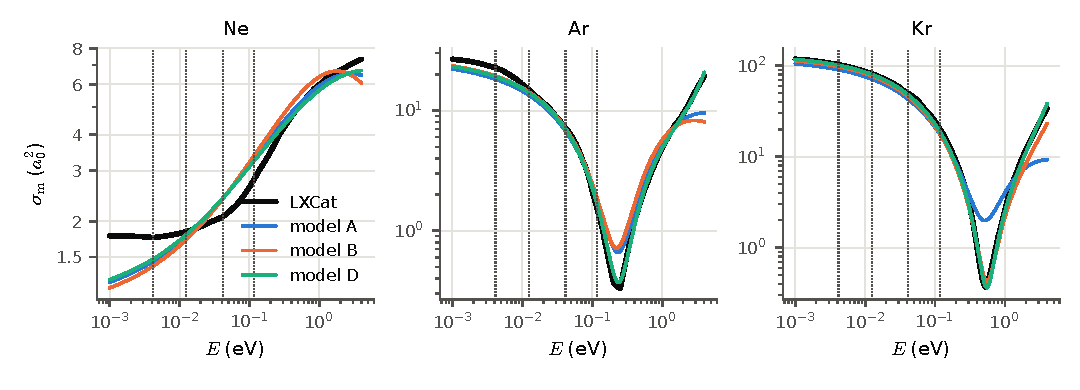
\includegraphics[width=\textwidth]{chapters/ea/fig_sigma.pdf}
\end{center}
\caption{Momentum-transfer cross sections of the LXCat sets used by the
classical kernel and of the three model families. The vertical lines mark the
photon energies of 1, 3, 10 and 28.3~THz.}
\label{ea:fig:sigma}
\end{figure}

\subsection{Numerical method}
\label{ea:sec:numerics}
{\noindent}(1) The radial equation is integrated by the method of Numerov,
on a uniform grid of step $0.01\,a_0$ for the smooth cores and on the
logarithmic grid $r=e^x$, $u=e^{x/2}y$, with
$y''=[(l+\frac12)^2+r^2(2V-k^2)]y$ and step $\Delta x=5\times10^{-4}$, for the
Coulomb-like cores of D. At $r_{\max}=400\,a_0$ the solution is matched to the
Riccati--Bessel functions, which fixes $\delta_l$ and the amplitude, and the
acceleration integrals of Eq.~\eqref{ea:eq:Racc} are accumulated during the
integration and normalized at the end. Partial waves up to $l=12$ are kept.

{\noindent}(2) For the deep models, halving the step, doubling $r_{\max}$ and
raising the largest $l$ to 16 change $G$ by at most $1.4\times10^{-5}$. The
cores of the models A reach $6\times10^{10}$ hartree in krypton, where the
recursion of Numerov is unstable on the uniform grid. The outward growth of the
solution through the forbidden core filters that error out. Starting instead
at a hard wall placed where $h^2\cdot2mV/\hbar^2$ last exceeds 2, with half the
step, changes $G$ of the models A and B by at most $1\times10^{-5}$. The force
identity holds as stated in Sec.~\ref{ea:sec:force}, and detailed balance,
Eq.~\eqref{ea:eq:db}, to $10^{-13}$.

\subsection{The free--free Gaunt factor}
\label{ea:sec:gaunt}
{\noindent}(1) Figure~\ref{ea:fig:G} shows $G=\sigma_+/\sigma_+^{\rm soft}$ for the
deep models. For $\hbar\omega\ll E$ it tends to one, with the slope
$1+\frac12\,\dd\ln\sm/\dd\ln E$ in $\hbar\omega/E$ that Eq.~\eqref{ea:eq:firstorder}
predicts. Below $E\approx\hbar\omega$ it grows as $E^{-3/2}$. There the final
state is near $\hbar\omega$ whatever the initial energy, $\sigma_+$ varies as
$1/k$, and the soft-photon reference vanishes as $k^2$.

\begin{figure}[ht]
\begin{center}
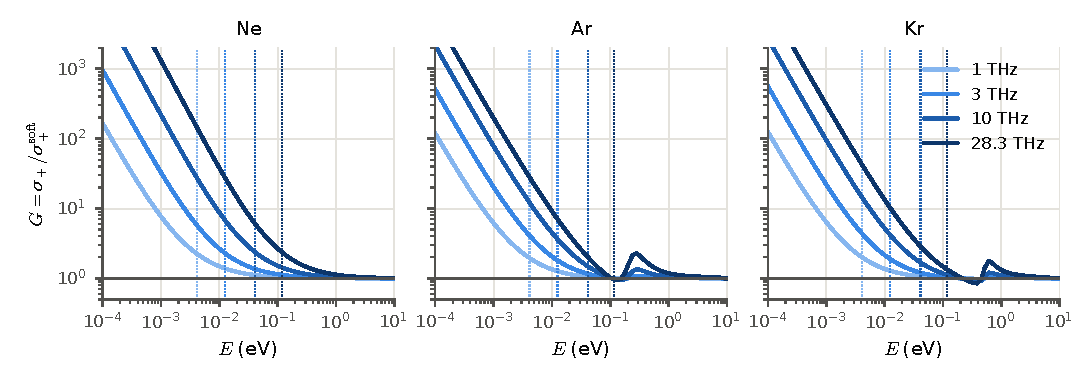
\includegraphics[width=\textwidth]{chapters/ea/fig_G.pdf}
\end{center}
\caption{The free--free Gaunt factor $G=\sigma_+/\sigma_+^{\rm soft}$ of the deep
models at 1, 3, 10 and 28.3~THz. The dotted lines mark $E=\hbar\omega$.}
\label{ea:fig:G}
\end{figure}

{\noindent}(2) A code that needs $\sigma_+$ without solving the scattering
problem can use one of three forms built on $\sm$ alone, the two-energy form of
Eq.~\eqref{ea:eq:twoenergy}, the mean-energy form of Eq.~\eqref{ea:eq:firstorder},
or the mean-momentum form of Eq.~\eqref{ea:eq:meanmom} with the true $\sm$.
Table~\ref{ea:tab:presc} compares them with the exact result of each deep model.
The two-energy form, exact for the zero-range potential, overestimates
$\sigma_+$ of argon by a factor 2.1 for thermal electrons at 28.3~THz. The
polarization tail makes the $p$ wave matter at low energy, since it raises
the $p$-wave phase shift as $\pi\alpha_dk^2/15$ in atomic units rather than as
$k^3$ \cite{ea:OMalleySpruchRosenberg1961}, a law the check script confirms for
the deep models. The mean-energy form falls up to 25\,\% short there.

{\noindent}(3) The mean-momentum form is the best of the three. For neon it
is within 0.5\,\% of the exact result at every energy above $\hbar\omega$ up to
28.3~THz. For argon and krypton it is within 1.2\,\% at 3~THz and 3.3\,\% at
10~THz above $\hbar\omega$. At 28.3~THz it errs by up to 14\,\% in argon and
17\,\% in krypton above $\hbar\omega$, most where the final energy
$E+\hbar\omega$ falls at the Ramsauer minimum of the model, 0.24~eV in argon
and 0.55~eV in krypton. There $\sm$ changes by a large factor across one photon
energy. Table~\ref{ea:tab:presc} shows errors of the same size for thermal
electrons below $\hbar\omega$. In the thermal
averages of Sec.~\ref{ea:sec:thermal} up to 4~THz the form is within 1\,\% of the
exact result for every gas.

\begin{table}[ht]
\caption{The exact Gaunt factor $G$ of the deep models at $E=26$~meV and
0.3~eV, and the two-energy (TE), mean-energy (ME) and mean-momentum (MM) forms
with the model's own $\sm$, as ratios to the exact cross section.}
\label{ea:tab:presc}
\begin{center}
\begin{tabular}{lccccccc}
\toprule
 & & \multicolumn{4}{c}{$E=26$~meV} & \multicolumn{2}{c}{$E=0.3$~eV}\\
gas & $f$ (THz) & $G$ & TE & ME & MM & $G$ & MM\\
\midrule
\tabinput{chapters/ea/tab_presc.tex}
\bottomrule
\end{tabular}
\end{center}
\end{table}

\subsection{Polarization bremsstrahlung}
\label{ea:sec:pbnum}
{\noindent}(1) The term of Eq.~\eqref{ea:eq:pb-op} has the same angular structure
as $\rv$, so in the acceleration form it adds $-m\omega^2\alpha_d/r^2$ to
$V'(r)$. With the cut-off $r^2\to r^2+r_c^2$ of the polarization potential of
model D, Table~\ref{ea:tab:pb} gives the change of $\sigma_+$. It is below 0.7\,\%
up to 3~THz for every gas and energy. At 28.3~THz it reaches $-13$\,\% for slow
electrons in argon, $-8$\,\% in krypton and $+4$\,\% in neon, so a CO$_2$-laser
calculation for a cold gas has to include it. At 1~eV it stays below 1\,\% at
every frequency. Geltman \cite{ea:Geltman1995} studied the same field-induced
dipole in the laser-assisted elastic scattering of Sec.~\ref{ea:sec:strong}.

\begin{table}[ht]
\caption{Change of $\sigma_+$ in percent when the polarization bremsstrahlung
of Eq.~\eqref{ea:eq:pb-op} is added, for the deep models.}
\label{ea:tab:pb}
\begin{center}
\begin{tabular}{lccccc}
\toprule
gas & $E$ (meV) & 1~THz & 3~THz & 10~THz & 28.3~THz\\
\midrule
\tabinput{chapters/ea/tab_pb.tex}
\bottomrule
\end{tabular}
\end{center}
\end{table}

\section{Thermal absorption and the error of the classical kernel}
\label{ea:sec:thermal}

\subsection{The pure gases}
{\noindent}(1) Equation~\eqref{ea:eq:R} gives $\mathcal R(T,\omega)$ from $G$ and
$\sm$ of each model. Table~\ref{ea:tab:R} lists it for the deep models with the
range over the three families. Up to 4~THz the classical kernel is right to
2.5\,\% or better for every gas and temperature, and to 2.8\,\% with any of the
three families. At 10~THz electrons at 300~K
absorb 12\,\% less than the classical kernel says in argon and 7\,\% less in
krypton, and at 28.3~THz 41\,\% and 25\,\% less. In neon the two effects of
Sec.~\ref{ea:sec:soft} cancel to within 3\,\%. Above 0.3~eV the classical kernel
is right to 1.6\,\% at every frequency up to 28.3~THz.

\begin{table}[ht]
\caption{The ratio $\mathcal R=\kappa/\kappa_{\rm cl}$ of Eq.~\eqref{ea:eq:R} for
each gas, from the deep model D, and its range over the models A, B and D.}
\label{ea:tab:R}
\begin{center}
\begin{tabular}{lccccccc}
\toprule
 & & \multicolumn{2}{c}{$T=300$~K} & \multicolumn{2}{c}{$T=0.1$~eV} & \multicolumn{2}{c}{$T=0.63$~eV}\\
gas & $f$ (THz) & D & A--D & D & A--D & D & A--D\\
\midrule
\tabinput{chapters/ea/tab_R.tex}
\bottomrule
\end{tabular}
\end{center}
\end{table}

\subsection{The two fills}
{\noindent}(1) In a mixture each gas contributes to $\kappa_{\rm cl}$ in
proportion to its share $x_g\langle v^3\sm\rangle$, and the ratio of the
mixture is the share-weighted mean of the ratios of its gases. Fluorine
appears only at 0.2 and 0.3\,\%, and its molecular cross section is treated
with the mean-momentum form. At 300~K krypton carries 44\,\% of the classical
absorption of the neon fill and 83\,\% of that of the argon fill, because per
atom its $\langle v^3\sm\rangle$ is 15 times that of neon and 7.6 times that of
argon.

{\noindent}(2) Table~\ref{ea:tab:fills} gives the ratio for both fills, from the
deep models and, in parentheses, from the mean-momentum form with the measured
cross sections alone. Figure~\ref{ea:fig:R} shows it against frequency.

\begin{table}[ht]
\caption{The ratio $\mathcal R=\kappa/\kappa_{\rm cl}$ for the two fills of
Sec.~\ref{ea:sec:why}, from the deep models, and in parentheses from the
mean-momentum form with the LXCat cross sections.}
\label{ea:tab:fills}
\begin{center}
\begin{tabular}{lccccc}
\toprule
fill & $f$ (THz) & $T=300$~K & $T=0.1$~eV & $T=0.63$~eV & $T=1.08$~eV\\
\midrule
\tabinput{chapters/ea/tab_fills.tex}
\bottomrule
\end{tabular}
\end{center}
\end{table}

\begin{figure}[ht]
\begin{center}
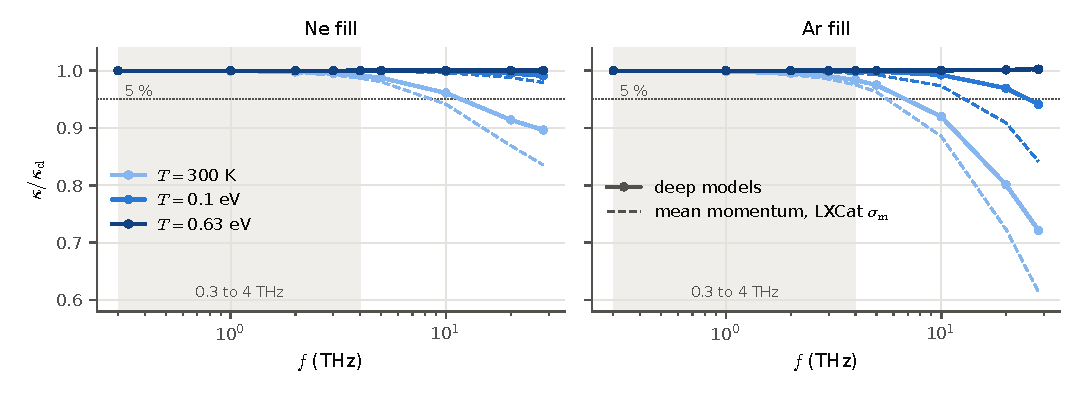
\includegraphics[width=\textwidth]{chapters/ea/fig_R_v2.pdf}
\end{center}
\caption{The ratio of the quantum to the classical absorption coefficient for
the two fills against frequency. Solid lines are the deep models, dashed lines
the mean-momentum form with the LXCat cross sections. The shaded band is the
band of 0.3 to 4~THz proposed for reheating.}
\label{ea:fig:R}
\end{figure}

\subsection{The answer for the laser gas}
{\noindent}(1) In the band of 0.3 to 4~THz proposed for reheating, the
classical kernel differs from the quantum result by
at most 1.6\,\% in either fill at any electron temperature from 300~K to
1.08~eV. The mean-momentum form with the measured cross sections gives at most
2.5\,\%. Both are below the 5\,\% of the criterion of Sec.~\ref{ea:sec:why}, so
the classical kernel holds in that band, and the absorption lengths and
reflectances computed with it stand.

{\noindent}(2) For a CO$_2$ laser on a thermalized fill the classical kernel
fails. At 28.3~THz and 300~K the quantum absorption is 10\,\% below it in the
neon fill and 28\,\% below it in the argon fill, before the polarization
bremsstrahlung of Sec.~\ref{ea:sec:pbnum}. Above 0.3~eV it is right to 1\,\% in
both fills at every frequency studied. A code that heats electrons at such
frequencies should multiply the classical absorption by $\mathcal R$, or
replace the diffusion term of the two-term equation by the jump operator of
Eq.~\eqref{ea:eq:jump} with the mean-momentum cross section.

\section{Electron--ion or electron--atom}
\label{ea:sec:ei}

{\noindent}(1) The ions contribute the effective collision frequency
$\nu_T\Lambda$ \cite{ea:Atzeni2004}, with
\[
\nu_T=\frac{4\sqrt{2\pi}}{3}\,\frac{n_iZ^2e^4}{m^{1/2}(\kB T)^{3/2}},\qquad
\Lambda=\frac{\pi}{\sqrt3}\,\langle g\rangle\,\frac{1-e^{-u}}{u},
\]
the thermal Gaunt factor $\langle g\rangle$ times the factor of stimulated emission
\cite{ea:Kramers1923,ea:KarzasLatter1961}. The atoms
contribute $\kappa$ of Eq.~\eqref{ea:eq:kappa-mb}, which corresponds to the
effective collision frequency $(mN/3\kB T)\langle v^3\sm\rangle\mathcal R$.
With singly charged ions, $n_i=n_e$, the ions win above the electron density at
which the two are equal.

{\noindent}(2) In the Born approximation the thermal Gaunt factor is
$\langle g\rangle=(\sqrt3/\pi)e^{u/2}K_0(u/2)$ \cite{ea:KarzasLatter1961}, valid for
$Ze^2/\hbar v\ll1$. For an electron of energy
$\kB T$, $Ze^2/\hbar v$ is 23 at 300~K and 3.5 at 1.08~eV, and the collisions
are classical. For $x=\omega Ze^2/mv^3\ll1$ and $\hbar\omega\ll\kB T$ the
classical thermal Gaunt factor is that of Scheuer \cite{ea:Scheuer1960},
$\langle g\rangle=(\sqrt3/\pi)\{\ln[(2\kB T)^{3/2}/\pi Ze^2m^{1/2}f]-\frac52\gamma\}$,
with $f$ in hertz. At 300~K and 1~THz, $x$ is about 5 for $v=(\kB T/m)^{1/2}$,
and that formula turns negative. For larger $x$ the classical Gaunt factor
tends to Kramers' value one from above. The estimate used here is the larger
of Scheuer's value and one. At 1~THz, where $u\le0.16$, the Born value exceeds
this estimate at every temperature and bounds the ionic absorption from
above. At 28.3~THz and 300~K, where $u=4.5$, the Born value falls to 0.44,
below Kramers' one, which is then the better estimate.

{\noindent}(3) Table~\ref{ea:tab:ei} and Fig.~\ref{ea:fig:ei} give the density
at which the two kinds of absorption are equal at 1~THz. Ions dominate only in
a cold and dense plasma. At 300~K that takes $7.0\times10^{19}$~m$^{-3}$ in the
neon fill and $1.5\times10^{20}$~m$^{-3}$ in the argon fill with the classical
Gaunt factor, and at 0.63~eV more than $10^{22}$~m$^{-3}$ in both. At 28.3~THz
and 300~K, with Kramers' one, the densities are $2.7\times10^{20}$ and
$4.5\times10^{20}$~m$^{-3}$. The plasma of the laser gas with the beam on,
$2.7\times10^{21}$~m$^{-3}$ at 1.08~eV, absorbs on atoms, and so does the
afterglow while its electrons stay warm. In a thermalized afterglow at
$10^{20}$~m$^{-3}$ and 1~THz the ions absorb 1.4 times as much as the atoms in
the neon fill and 0.7 times as much in the argon fill. The atoms dominate
because $n_e/N$ is small only away from that corner.

\begin{table}[ht]
\caption{Electron density in m$^{-3}$ at which electron--ion and electron--atom
absorption are equal at 1~THz, with the classical estimate of the thermal
Gaunt factor and with the Born value \cite{ea:KarzasLatter1961}. Ions dominate above it.}
\label{ea:tab:ei}
\begin{center}
\begin{tabular}{lccccc}
\toprule
fill & $T$ (eV) & $\langle g\rangle_{\rm cl}$ & $\langle g\rangle_{\rm Born}$ & $n_e$, classical & $n_e$, Born\\
\midrule
\tabinput{chapters/ea/tab_ei.tex}
\bottomrule
\end{tabular}
\end{center}
\end{table}

\begin{figure}[ht]
\begin{center}
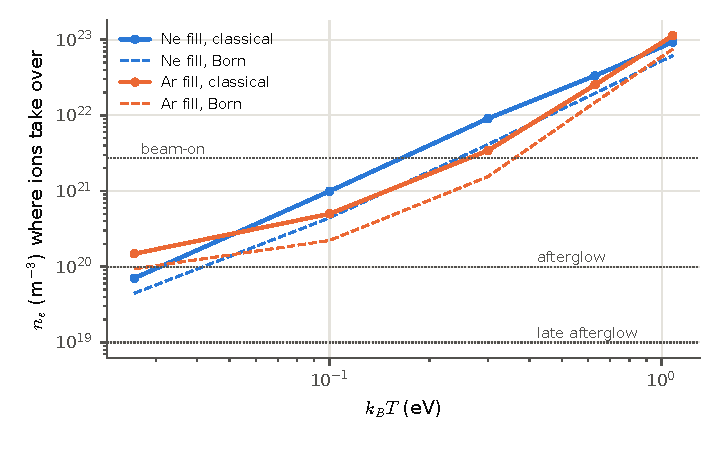
\includegraphics[width=0.75\textwidth]{chapters/ea/fig_ei.pdf}
\end{center}
\caption{The electron density above which electron--ion absorption exceeds
electron--atom absorption at 1~THz. Solid lines use the classical estimate of
the Gaunt factor, dashed lines the Born value. The horizontal lines mark the
electron density of the laser gas with the beam on, $2.7\times10^{21}$~m$^{-3}$,
and in the afterglow, $10^{20}$ and $10^{19}$~m$^{-3}$.}
\label{ea:fig:ei}
\end{figure}

\section{Summary}
\label{ea:sec:summary}

{\noindent}(1) The one-photon free--free cross section of an electron in the
field of an atom is Eq.~\eqref{ea:eq:sigplus}, a sum over partial waves of the
squared dipole integrals, which the acceleration form, Eq.~\eqref{ea:eq:Racc},
makes absolutely convergent. Emission follows from detailed balance,
Eq.~\eqref{ea:eq:db}, and the absorption coefficient of Maxwell electrons carries
the factor $1-e^{-u}$, Eq.~\eqref{ea:eq:kappa-mb}. The kinetic equation is the jump
operator of Eq.~\eqref{ea:eq:jump}, whose Fokker--Planck limit,
Eq.~\eqref{ea:eq:Dfp}, is the field term of the two-term Boltzmann equation at
$\omega\gg\nu$.

{\noindent}(2) The force identity, Eq.~\eqref{ea:eq:force}, reduces the soft-photon
limit to the momentum-transfer cross section, Eq.~\eqref{ea:eq:soft}, and the
classical limit is the Lorentz gas, Eq.~\eqref{ea:eq:kappa-cl}. The cross section
that belongs in the classical formula is therefore $\sm$, which settles the
choice between $\sm$ and the elastic cross section that the literature on
neutral bremsstrahlung leaves open \cite{ea:Buzulutskov2018}.

{\noindent}(3) At finite photon energy the cross section is known exactly for
a zero-range potential, Eq.~\eqref{ea:eq:twoenergy}, which is also the emission
formula of neutral bremsstrahlung, Eq.~\eqref{ea:eq:nbrs}, and in Born
approximation, Eq.~\eqref{ea:eq:meanmom}. Both agree to first order with
Eq.~\eqref{ea:eq:firstorder}, and the model potentials confirm that this order is
universal. Wherever $\hbar\omega\le E$ the mean-momentum form with the true
$\sm$ is accurate to 0.5\,\% for neon at every frequency and to 3.3\,\% for
argon and krypton up to 10~THz, but errs by up to 17\,\% at 28.3~THz near the
Ramsauer minima.

{\noindent}(4) For the laser gas the quantum correction to the classical
kernel is below 1.6\,\% from 0.3 to 4~THz at every temperature, so the
classical kernel holds in that band. It becomes $-10$ to $-28$\,\% at 28.3~THz for electrons at 300~K, where
polarization bremsstrahlung changes the cross section of slow electrons by up
to $-13$\,\%. Electron--ion absorption competes only in a cold afterglow above
about $10^{20}$~m$^{-3}$.

{\noindent}(5) Left open are the exchange of the scattering electron with the
atomic electrons, which a one-body potential only mimics and which the
multichannel R-matrix calculation of Bell and Berrington
\cite{ea:BellBerrington1987} treats for argon, the molecular fluorine, and the
laser-assisted measurements on argon that find photon exchange, up to 12\,\%
of the field-free cross section, where the theory of Kroll and Watson predicts
none \cite{ea:WallbankHolmes1993,ea:WallbankHolmes1994}. The
measured neutral bremsstrahlung \cite{ea:TaylorCaledonia1969,ea:Ranson1977} is the
experimental test of the models at higher photon energies.

\chapterappendix
\section{Partial waves}
\label{ea:app:angular}

{\noindent}(1) Take $\ehat=\hat z$, which the average over the direction of
the electron allows. The matrix elements of $\cos\theta$ are
$\langle l+1,m|\cos\theta|lm\rangle=[((l+1)^2-m^2)/((2l+1)(2l+3))]^{1/2}$ and
vanish for $m'\ne m$. Summing over $m$,
\begin{equation}
\sum_{m=-l}^l\frac{(l+1)^2-m^2}{(2l+1)(2l+3)}
=\frac{(2l+1)(l+1)^2-l(l+1)(2l+1)/3}{(2l+1)(2l+3)}=\frac{l+1}{3},
\end{equation}
and the same steps with $\langle l-1,m|\cos\theta|lm\rangle^2=(l^2-m^2)/((2l-1)(2l+1))$
give $l/3$, which is Eq.~\eqref{ea:eq:angsum}.

{\noindent}(2) The elastic amplitude is
$f(\theta)=k^{-1}\sum_l(2l+1)e^{i\delta_l}\sin\delta_l\,P_l(\cos\theta)$.
In $\int(1-\cos\theta)|f|^2\dd\Omega$ the term with $1$ gives
$(4\pi/k^2)\sum_l(2l+1)\sin^2\delta_l$, and with
$\cos\theta\,P_l=[(l+1)P_{l+1}+lP_{l-1}]/(2l+1)$ the term with $\cos\theta$
gives $(4\pi/k^2)\sum_l2(l+1)\sin\delta_l\sin\delta_{l+1}\cos(\delta_l-\delta_{l+1})$.
Their difference, with
$\sin^2\delta_l+\sin^2\delta_{l+1}-2\sin\delta_l\sin\delta_{l+1}\cos(\delta_l-\delta_{l+1})
=\sin^2(\delta_l-\delta_{l+1})$ and $(2l+1)=(l+1)+l$ regrouped, is
Eq.~\eqref{ea:eq:sigmam}.

\section{The integrals of the zero-range limit}
\label{ea:app:abel}

{\noindent}(1) With $\hat\jmath_1(x)=\sin x/x-\cos x$ and the factor
$e^{-\eta r}$,
\begin{equation}
\int_0^\infty\hat\jmath_1(k'r)\,r\cos(kr)\,e^{-\eta r}\dd r
=\frac1{k'}\int_0^\infty\sin(k'r)\cos(kr)e^{-\eta r}\dd r
-\int_0^\infty r\cos(k'r)\cos(kr)e^{-\eta r}\dd r .
\end{equation}

{\noindent}(2) The first integral is
$\frac1{2k'}\int[\sin(k'+k)r+\sin(k'-k)r]e^{-\eta r}\dd r\to
\frac1{2k'}\big[\frac1{k'+k}+\frac1{k'-k}\big]=\frac{1}{k'^2-k^2}$.

{\noindent}(3) With $\int_0^\infty r\cos(qr)e^{-\eta r}\dd r
=(\eta^2-q^2)/(\eta^2+q^2)^2\to-1/q^2$, the second integral tends to
$-\frac12\big[(k'-k)^{-2}+(k'+k)^{-2}\big]=-(k^2+k'^2)/(k'^2-k^2)^2$.

{\noindent}(4) The difference is
$[(k'^2-k^2)+(k'^2+k^2)]/(k'^2-k^2)^2=2k'^2/(k'^2-k^2)^2$, which is
Eq.~\eqref{ea:eq:abel}. The integral with $\sin kr$ in place of $\cos kr$ tends
to zero for $k\ne k'$, since $\int\sin a r\sin b r\,e^{-\eta r}\dd r$ and
$\int r\sin(qr)e^{-\eta r}\dd r=2\eta q/(\eta^2+q^2)^2$ both vanish with $\eta$.

\section{The numerical checks}
\label{ea:app:checks}

{\noindent}(1) A check script computes every boxed result of these notes and
reproduces every number printed in them, from the tables it writes and from
the prose. It needs numpy, scipy and the LXCat cross sections, runs about
three minutes, and stops with an error if any check fails. The model
potentials are fitted by a second script, and the check script verifies that
the stored parameters reproduce the fit quality and the scattering lengths of
Table~\ref{ea:tab:models}.

{\noindent}(2) It uses four methods. Identities are verified against
independent evaluations, the golden-rule cross section against the plane-wave
Born formula and the Born mean-momentum form to $10^{-14}$. Limits are
verified by their convergence, the zero-range form by narrowing the well and
the soft-photon and Fokker--Planck limits by the order of the remainder. The
numerics are verified by halving the steps and doubling the ranges. The tables
and the numbers in the text are printed from the same computation, and the
script recomputes each number of the prose to the digits shown.

\begin{longtable}{L{4.0cm}cccc}
\caption{The numerical checks of these notes, by the equation, table or section they verify. The second column counts all checks of the row, the third gives the largest deviation among its quantitative checks, relative except for the slopes of Eq.~(\ref*{ea:eq:soft}), which are absolute, the fourth counts the numbers printed in these notes that the script reproduces to their last digit, and the fifth the logical conditions.}\label{ea:tab:checks}\\
\toprule
Equation & Checks & Largest deviation & Printed & Logical\\
\midrule
\endfirsthead
\toprule
Equation & Checks & Largest deviation & Printed & Logical\\
\midrule
\endhead
\bottomrule
\endfoot
Eq.~(\ref*{ea:eq:sigplus}) & 4 & $2.3\times10^{-15}$ &  & \\
Eq.~(\ref*{ea:eq:angsum}) & 8 & $4.4\times10^{-16}$ &  & \\
Eq.~(\ref*{ea:eq:abel}) & 4 & $4.4\times10^{-10}$ &  & \\
Eq.~(\ref*{ea:eq:R01}) & 4 & $1.1\times10^{-2}$ &  & 1\\
Eq.~(\ref*{ea:eq:twoenergy}) & 3 & $4.7\times10^{-16}$ &  & \\
Eq.~(\ref*{ea:eq:nbrs}) & 3 & $1.2\times10^{-16}$ &  & \\
Eq.~(\ref*{ea:eq:db}) & 8 & $8.5\times10^{-14}$ &  & \\
Eq.~(\ref*{ea:eq:kappa-mb}) & 3 & $1.4\times10^{-7}$ &  & \\
Eq.~(\ref*{ea:eq:Dfp}) & 6 & $6.7\times10^{-16}$ &  & \\
Eq.~(\ref*{ea:eq:jump}) & 4 & $6.6\times10^{-5}$ &  & 1\\
Eq.~(\ref*{ea:eq:force}) & 4 & $9.2\times10^{-5}$ &  & \\
Eq.~(\ref*{ea:eq:sigmam}) & 6 & $5.1\times10^{-8}$ &  & \\
Eq.~(\ref*{ea:eq:soft}) & 12 & $5.9\times10^{-3}$ &  & 6\\
Eq.~(\ref*{ea:eq:kappa-cl}) & 4 & $6.9\times10^{-5}$ &  & \\
Eq.~(\ref*{ea:eq:meanmom}) & 4 & $1.6\times10^{-15}$ &  & \\
Eq.~(\ref*{ea:eq:firstorder}) & 6 &  &  & 6\\
Sec.~\ref*{ea:sec:strong} & 9 & $2.0\times10^{-16}$ & 4 & 1\\
Table~\ref*{ea:tab:weak} & 1 &  &  & 1\\
Sec.~\ref*{ea:sec:models} & 50 & $2.6\times10^{-5}$ & 6 & 14\\
Sec.~\ref*{ea:sec:numerics} & 6 & $1.4\times10^{-5}$ & 3 & 1\\
Sec.~\ref*{ea:sec:gaunt} & 20 & $2.2\times10^{-4}$ & 8 & 6\\
Table~\ref*{ea:tab:presc} & 5 &  &  & 5\\
Table~\ref*{ea:tab:pb} & 1 &  &  & 1\\
Sec.~\ref*{ea:sec:thermal} & 22 &  & 15 & 7\\
Sec.~\ref*{ea:sec:ei} & 14 &  & 10 & 4\\
Sec.~\ref*{ea:sec:why} & 11 &  & 11 & \\
Sec.~\ref*{ea:sec:ham} & 5 &  & 5 & \\
Sec.~\ref*{ea:sec:pb} & 1 &  &  & 1\\
Sec.~\ref*{ea:sec:cross} & 1 &  &  & 1\\
Sec.~\ref*{ea:sec:born} & 1 &  &  & 1\\
Sec.~\ref*{ea:sec:force} & 2 &  & 1 & 1\\
Sec.~\ref*{ea:sec:soft} & 2 &  & 2 & \\
Sec.~\ref*{ea:sec:zerorange} & 2 &  & 2 & \\
Sec.~\ref*{ea:sec:firstorder} & 2 &  & 2 & \\
Sec.~\ref*{ea:sec:pbnum} & 4 &  & 3 & 1\\
\midrule
Total & 242 & & 72 & 59\\
\end{longtable}


\raggedright
\begin{thebibliography}{99}
\bibitem{ea:Atzeni2004} S.~Atzeni and J.~Meyer-ter-Vehn, \emph{The Physics of Inertial Fusion}
(Oxford University Press, Oxford, 2004), doi:\href{https://doi.org/10.1093/acprof:oso/9780198562641.001.0001}{10.1093/acprof:oso/9780198562641.001.0001}.
\bibitem{ea:Kramers1923} H.~A.~Kramers, Phil. Mag. \textbf{46}, 836 (1923), doi:\href{https://doi.org/10.1080/14786442308565244}{10.1080/14786442308565244}.
\bibitem{ea:KarzasLatter1961} W.~J.~Karzas and R.~Latter, Astrophys. J. Suppl. \textbf{6}, 167 (1961), doi:\href{https://doi.org/10.1086/190063}{10.1086/190063}.
\bibitem{ea:BunkinFedorov1966} F.~V.~Bunkin and M.~V.~Fedorov, \emph{Bremsstrahlung in a
strong radiation field}, Sov.\ Phys.\ JETP \textbf{22}, 844 (1966), record at
\url{http://www.jetp.ras.ru/cgi-bin/e/index/e/22/4/p844?a=list}.
\bibitem{ea:Margenau1946} H.~Margenau, Phys. Rev. \textbf{69}, 508 (1946), doi:\href{https://doi.org/10.1103/physrev.69.508}{10.1103/physrev.69.508}.
\bibitem{ea:KasyanovStarostin1965} V.~Kas'yanov and A.~Starostin, \emph{On the
theory of bremsstrahlung of slow electrons on atoms}, Sov.\ Phys.\ JETP
\textbf{21}, 193 (1965), record at
\url{http://www.jetp.ras.ru/cgi-bin/e/index/e/21/1/p193?a=list}.
\bibitem{ea:Low1958} F.~E.~Low, Phys. Rev. \textbf{110}, 974 (1958), doi:\href{https://doi.org/10.1103/physrev.110.974}{10.1103/physrev.110.974}.
\bibitem{ea:BurnettKroll1968} T.~H.~Burnett and N.~M.~Kroll, Phys. Rev. Lett. \textbf{20}, 86 (1968), doi:\href{https://doi.org/10.1103/physrevlett.20.86}{10.1103/physrevlett.20.86}.
\bibitem{ea:KrollWatson1973} N.~M.~Kroll and K.~M.~Watson, Phys. Rev. A \textbf{8}, 804 (1973), doi:\href{https://doi.org/10.1103/physreva.8.804}{10.1103/physreva.8.804}.
\bibitem{ea:DalgarnoLane1966} A.~Dalgarno and N.~F.~Lane, ApJ \textbf{145}, 623 (1966), doi:\href{https://doi.org/10.1086/148801}{10.1086/148801}.
\bibitem{ea:OhmuraOhmura1960} T.~Ohmura and H.~Ohmura, ApJ \textbf{131}, 8 (1960), doi:\href{https://doi.org/10.1086/146799}{10.1086/146799}.
\bibitem{ea:Geltman1973} S.~Geltman, J. Quant. Spectrosc. Radiat. Transf. \textbf{13}, 601 (1973), doi:\href{https://doi.org/10.1016/0022-4073(73)90019-8}{10.1016/0022-4073(73)90019-8}.
\bibitem{ea:BellBerrington1987} K.~L.~Bell and K.~A.~Berrington, J. Phys. B: At. Mol. Phys. \textbf{20}, 1329 (1987), doi:\href{https://doi.org/10.1088/0022-3700/20/6/017}{10.1088/0022-3700/20/6/017}.
\bibitem{ea:TaylorCaledonia1969} R.~L.~Taylor and G.~Caledonia, J. Quant. Spectrosc. Radiat. Transf. \textbf{9}, 657 (1969), doi:\href{https://doi.org/10.1016/0022-4073(69)90013-2}{10.1016/0022-4073(69)90013-2}.
\bibitem{ea:Ranson1977} P.~Ranson, O.~Vall\'ee and J.~Chapelle, Rev. Phys. Appl. (Paris) \textbf{12}, 1829 (1977), doi:\href{https://doi.org/10.1051/rphysap:0197700120120182900}{10.1051/rphysap:0197700120120182900}.
\bibitem{ea:Buzulutskov2018} A.~Buzulutskov \emph{et al.}, Astropart. Phys. \textbf{103}, 29 (2018), doi:\href{https://doi.org/10.1016/j.astropartphys.2018.06.005}{10.1016/j.astropartphys.2018.06.005}.
\bibitem{ea:Weingartshofer1977} A.~Weingartshofer \emph{et al.}, Phys. Rev. Lett. \textbf{39}, 269 (1977), doi:\href{https://doi.org/10.1103/physrevlett.39.269}{10.1103/physrevlett.39.269}.
\bibitem{ea:WallbankHolmes1993} B.~Wallbank and J.~K.~Holmes, Phys. Rev. A \textbf{48}, R2515 (1993), doi:\href{https://doi.org/10.1103/physreva.48.r2515}{10.1103/physreva.48.r2515}.
\bibitem{ea:WallbankHolmes1994} B.~Wallbank and J.~K.~Holmes, J. Phys. B: At. Mol. Opt. Phys. \textbf{27}, 5405 (1994), doi:\href{https://doi.org/10.1088/0953-4075/27/21/027}{10.1088/0953-4075/27/21/027}.
\bibitem{ea:Geltman1995} S.~Geltman, Phys. Rev. A \textbf{51}, R34 (1995), doi:\href{https://doi.org/10.1103/physreva.51.r34}{10.1103/physreva.51.r34}.
\bibitem{ea:OMalleySpruchRosenberg1961} T.~F.~O'Malley, L.~Spruch and L.~Rosenberg, J. Math. Phys. \textbf{2}, 491 (1961), doi:\href{https://doi.org/10.1063/1.1703735}{10.1063/1.1703735}.
\bibitem{ea:Schwerdtfeger2019} P.~Schwerdtfeger and J.~K.~Nagle, Mol. Phys. \textbf{117}, 1200 (2019), doi:\href{https://doi.org/10.1080/00268976.2018.1535143}{10.1080/00268976.2018.1535143}.
\bibitem{ea:Kitajima2015} M.~Kitajima \emph{et al.}, J. Phys.: Conf. Ser. \textbf{635}, 012030 (2015), doi:\href{https://doi.org/10.1088/1742-6596/635/1/012030}{10.1088/1742-6596/635/1/012030}.
\bibitem{ea:Kurokawa2011} M.~Kurokawa \emph{et al.}, Phys. Rev. A \textbf{84}, 062717 (2011), doi:\href{https://doi.org/10.1103/physreva.84.062717}{10.1103/physreva.84.062717}.
\bibitem{ea:BuckmanMitroy1989} S.~J.~Buckman and J.~Mitroy, J. Phys. B: At. Mol. Opt. Phys. \textbf{22}, 1365 (1989), doi:\href{https://doi.org/10.1088/0953-4075/22/9/010}{10.1088/0953-4075/22/9/010}.
\bibitem{ea:OMalleyCrompton1980} T.~F.~O'Malley and R.~W.~Crompton, J. Phys. B: At. Mol. Phys. \textbf{13}, 3451 (1980), doi:\href{https://doi.org/10.1088/0022-3700/13/17/023}{10.1088/0022-3700/13/17/023}.
\bibitem{ea:GSZ1969} A.~E.~S.~Green, D.~L.~Sellin and A.~S.~Zachor, Phys. Rev. \textbf{184}, 1 (1969), doi:\href{https://doi.org/10.1103/physrev.184.1}{10.1103/physrev.184.1}.
\bibitem{ea:HagelaarPitchford2005} G.~J.~M.~Hagelaar and L.~C.~Pitchford, Plasma Sources Sci. Technol. \textbf{14}, 722 (2005), doi:\href{https://doi.org/10.1088/0963-0252/14/4/011}{10.1088/0963-0252/14/4/011}.
\bibitem{ea:Scheuer1960} P.~A.~G.~Scheuer, Mon. Not. R. Astron. Soc. \textbf{120}, 231 (1960), doi:\href{https://doi.org/10.1093/mnras/120.3.231}{10.1093/mnras/120.3.231}.
\bibitem{ea:LXCat} L.~C.~Pitchford \emph{et al.}, Plasma Process. Polym. \textbf{14}, 1600098 (2016), doi:\href{https://doi.org/10.1002/ppap.201600098}{10.1002/ppap.201600098}.
\end{thebibliography}
\endgroup
